%package list
\documentclass{article}
\usepackage[top=3cm, bottom=3cm, outer=3cm, inner=3cm]{geometry}
\usepackage{multicol}
\usepackage{graphicx}
\usepackage{url}
%\usepackage{cite}
\usepackage{hyperref}
\usepackage{array}
%\usepackage{multicol}
\newcolumntype{x}[1]{>{\centering\arraybackslash\hspace{0pt}}p{#1}}
\usepackage{natbib}
\usepackage{pdfpages}
\usepackage{multirow}
\usepackage[normalem]{ulem}
\useunder{\uline}{\ul}{}
\usepackage{svg}
\usepackage{xcolor}
\usepackage{listings}
\lstdefinestyle{ascii-tree}{
    literate={├}{|}1 {─}{--}1 {└}{+}1 
  }
\lstset{basicstyle=\ttfamily,
  showstringspaces=false,
  commentstyle=\color{red},
  keywordstyle=\color{blue}
}
%\usepackage{booktabs}
\usepackage{caption}
\usepackage{subcaption}
\usepackage{float}
\usepackage{array}

\newcolumntype{M}[1]{>{\centering\arraybackslash}m{#1}}
\newcolumntype{N}{@{}m{0pt}@{}}


%%%%%%%%%%%%%%%%%%%%%%%%%%%%%%%%%%%%%%%%%%%%%%%%%%%%%%%%%%%%%%%%%%%%%%%%%%%%
%%%%%%%%%%%%%%%%%%%%%%%%%%%%%%%%%%%%%%%%%%%%%%%%%%%%%%%%%%%%%%%%%%%%%%%%%%%%
\newcommand{\itemEmail}{rcompanocca@unsa.edu.pe}
\newcommand{\itemStudent}{Roni Companocca Checco}
\newcommand{\itemCourse}{Programación}
\newcommand{\itemCourseCode}{20210558}
\newcommand{\itemSemester}{II}
\newcommand{\itemUniversity}{Universidad Nacional de San Agustín de Arequipa}
\newcommand{\itemFaculty}{Facultad de Ingeniería de Producción y Servicios}
\newcommand{\itemDepartment}{Departamento Académico de Ingeniería de Sistemas e Informática}
\newcommand{\itemSchool}{Escuela Profesional de Ingeniería de Sistemas}
\newcommand{\itemAcademic}{2023 - B}
\newcommand{\itemInput}{Del 08 Diciembre 2023}
\newcommand{\itemOutput}{Al 13 Diciembre 2023}
\newcommand{\itemPracticeNumber}{21}
\newcommand{\itemTheme}{ Clases de Usuario
Herencia y Polimorfismo. Clases interfaces }
%%%%%%%%%%%%%%%%%%%%%%%%%%%%%%%%%%%%%%%%%%%%%%%%%%%%%%%%%%%%%%%%%%%%%%%%%%%%
%%%%%%%%%%%%%%%%%%%%%%%%%%%%%%%%%%%%%%%%%%%%%%%%%%%%%%%%%%%%%%%%%%%%%%%%%%%%

\usepackage[english,spanish]{babel}
\usepackage[utf8]{inputenc}
\AtBeginDocument{\selectlanguage{spanish}}
\renewcommand{\figurename}{Figura}
\renewcommand{\refname}{Referencias}
\renewcommand{\tablename}{Tabla} %esto no funciona cuando se usa babel
\AtBeginDocument{%
	\renewcommand\tablename{Tabla}
}

\usepackage{fancyhdr}
\pagestyle{fancy}
\fancyhf{}
\setlength{\headheight}{30pt}
\renewcommand{\headrulewidth}{1pt}
\renewcommand{\footrulewidth}{1pt}
\fancyhead[L]{\raisebox{-0.2\height}{
\includegraphics[width=3cm]{logo_episunsa.png}}}
\fancyhead[C]{\fontsize{7}{7}\selectfont	\itemUniversity \\ \itemFaculty \\ \itemDepartment \\ \itemSchool \\ \textbf{\itemCourse}}
\fancyhead[R]{\raisebox{-0.2\height}{
\includegraphics[width=1.2cm]{abet.png}}}
\fancyfoot[L]{Estudiante Roni Companocca Checco}
\fancyfoot[C]{\itemCourse}
\fancyfoot[R]{Página \thepage}

% para el codigo fuente
\usepackage{listings}
\usepackage{color, colortbl}
\definecolor{dkgreen}{rgb}{0,0.6,0}
\definecolor{gray}{rgb}{0.5,0.5,0.5}
\definecolor{mauve}{rgb}{0.58,0,0.82}
\definecolor{codebackground}{rgb}{0.95, 0.95, 0.92}
\definecolor{tablebackground}{rgb}{0.8, 0, 0}

\lstset{frame=tb,
	language=bash,
	aboveskip=3mm,
	belowskip=3mm,
	showstringspaces=false,
	columns=flexible,
	basicstyle={\small\ttfamily},
	numbers=none,
	numberstyle=\tiny\color{gray},
	keywordstyle=\color{blue},
	commentstyle=\color{dkgreen},
	stringstyle=\color{mauve},
	breaklines=true,
	breakatwhitespace=true,
	tabsize=3,
	backgroundcolor= \color{codebackground},
}

\begin{document}
	
	\vspace*{10px}
	
	\begin{center}	
		\fontsize{17}{17} \textbf{ Informe de Laboratorio \itemPracticeNumber}
	\end{center}
	\centerline{\textbf{\Large Tema: \itemTheme}}
	%\vspace*{0.5cm}	

	\begin{flushright}
		\begin{tabular}{|M{2.5cm}|N|}
			\hline 
			\rowcolor{tablebackground}
			\color{white} \textbf{Nota}  \\
			\hline 
			     \\[30pt]
			\hline 			
		\end{tabular}
	\end{flushright}	

	\begin{table}[H]
		\begin{tabular}{|x{4.7cm}|x{4.8cm}|x{4.8cm}|}
			\hline 
			\rowcolor{tablebackground}
			\color{white} \textbf{Estudiante} & \color{white}\textbf{Escuela}  & \color{white}\textbf{Asignatura}   \\
			\hline 
			{\itemStudent \par \itemEmail} & \itemSchool & {\itemCourse \par Semestre: \itemSemester \par Código: \itemCourseCode}     \\
			\hline 			
		\end{tabular}
	\end{table}		
	
	\begin{table}[H]
		\begin{tabular}{|x{4.7cm}|x{4.8cm}|x{4.8cm}|}
			\hline 
			\rowcolor{tablebackground}
			\color{white}\textbf{Laboratorio} & \color{white}\textbf{Tema}  & \color{white}\textbf{Duración}   \\
			\hline 
			\itemPracticeNumber & \itemTheme & 04 horas   \\
			\hline 
		\end{tabular}
	\end{table}
	
	\begin{table}[H]
		\begin{tabular}{|x{4.7cm}|x{4.8cm}|x{4.8cm}|}
			\hline 
			\rowcolor{tablebackground}
			\color{white}\textbf{Semestre académico} & \color{white}\textbf{Fecha de inicio}  & \color{white}\textbf{Fecha de entrega}   \\
			\hline 
			\itemAcademic & \itemInput &  \itemOutput  \\
			\hline 
		\end{tabular}
	\end{table}

    \section{TAREA}
	\begin{itemize}	
    \subsection{Objetivos:}
		\item Que el alumno demuestre poder crear “clases definidas por el programador”
		\item Implementar métodos para las clases definidas por el programador 
        \item Utilizar el mecanismo de Herencia de clases y polimorfismo
        \item Crear miembros de clase y de instancia según se requiera
        \item Crear clases interfaces que favorezcan la creación de jerarquías
        
       
    \subsection{Competencias a alcanzar:}
		\item Diseña, responsablemente, sistemas, componentes o procesos para satisfacer necesidades dentro de restricciones realistas: económicas, medio ambientales, sociales, políticas, éticas, de salud, de seguridad, manufacturación y sostenibilidad. 
        \item Aplica de forma flexible, técnicas, métodos, principios, normas, estándares y herramientas de ingeniería necesarias para la construcción de software e implementación de sistemas de información.
    \end{itemize}

    \section{EQUIPOS, MATERIALES Y TEMAS UTILIZADOS}
	\begin{itemize}
		\item Sistema Operativo Windows
		\item OpenJDK 64-Bits 17.0.7.
		\item Git 2.39.2.	
  	\item Cuenta en GitHub con el correo institucional.
	\end{itemize}

    \section{URL DE REPOSITORIO GITHUB}
	\begin{itemize}
		\item URL para el Repositorio GitHub.
		\item \url{https://github.com/RONI-COMPANOCCA-CHECCO}
		\item URL para el laboratorio 21 en el Repositorio GitHub.	
        \item \url{https://github.com/RONI-COMPANOCCA-CHECCO/FP2-LAB21}
	\end{itemize}
    
    \section{ACTIVIDADES}
	\begin{itemize}
      
        \item Crear diagrama de clases UML y programa

        \item Crear los miembros de cada clase de la forma más adecuada: de clase o de instancia
        
        \item Crear la clase Mapa, que esté constituida por el tablero antes visto, que posicione soldados en ciertas posiciones aleatorias (entre 1 y 10 soldados por cada ejército, sólo 1 ejército por reino). Se deben generar ejércitos de 2 reinos. No se admite guerra civil. El Mapa tiene como atributo el tipo de territorio que es (bosque, campo abierto, montaña, desierto, playa). La cantidad de soldados, así como todos sus atributos se deben generar aleatoriamente.

        \item Dibujar el Mapa con las restricciones que sólo 1 soldado como máximo en cada cuadrado.
        
        \item El mapa tiene un solo tipo de territorio.
        
        \item Considerar que el territorio influye en los resultados de las batallas, así cada reino tiene bonus según el territorio: Inglaterra->bosque, Francia->campo abierto, Castilla-Aragón->montaña, Moros->desierto, Sacro Imperio RomanoGermánico->bosque, playa, campo abierto. En dichos casos, se aumenta el nivel de vida en 1 a todos los soldados del reino beneficiado.

        \item En la historia, los ejércitos estaban conformados por diferentes tipos de soldados, que tenían similitudes, pero también particularidades.
        
        \item Basándose en la clase Soldado crear las clases Espadachín, Arquero, Caballero y Lancero. Las cuatro clases heredan de la superclase Soldado pero aumentan atributos y métodos, o sobrescriben métodos heredados.

        \item Los espadachines tienen como atributo particular "longitud de espada" y como acción "crear un muro de escudos" que es un tipo de defensa en particular.

        \item Los caballeros pueden alternar sus armas entre espada y lanza, además de desmontar (sólo se realiza cuando está montando e implica defender y cambiar de arma a espada), montar (sólo se realiza cuando está desmontado e implica montar, cambiar de arma a lanza y envestir). El caballero también puede envestir, ya sea montando o desmontando, cuando es desmontado equivale a atacar 2 veces pero cuando está montando implica a atacar 3 veces.

        \item Los arqueros tienen un número de flechas disponibles las cuales pueden dispararse y se gastan cuando se hace eso.

        \item Los lanceros tienen como atributo particular, "longitud de lanza" y como acción "schiltrom" (como una falange que es un tipo de defensa en particular y que aumenta su nivel de defensa en 1)

        \item Crear una clase abstracta, con métodos abstractos donde convenga. Usarla para implementar la jerarquía de herencia y la creación de las estructuras de datos

        \item Tendrá 2 Ejércitos que pueden ser constituidos sólo por espadachines caballeros, arqueros y lanceros. Crear una estructura de datos conveniente para cada ejército y para el tablero. Cada ejército tendrá n soldados aleatorios entre 1 y 10. Cada soldado tendrá un nombre autogenerado: Espadachin0X1, Arquero1X1, Caballero2X2, etc., un valor de nivel de vida autogenerado aleatoriamente, la fila y columna también autogenerados aleatoriamente (no puede haber 2 soldados en el mismo cuadrado) y valores autogenerados para el resto de atributos. Nivel de ataque y de defensa son aleatorios. Se debe mostrar el tablero con todos los soldados creados (usar caracteres como |  y otros) y distinguir los soldados de un ejército de los del otro ejército, y distinguir los tipos de soldado creados.
        
        \item Todos los caballeros tendrán los siguientes valores: ataque 13, defensa 7, nivel de vida [10..12]

        \item Todos los arqueros tendrán los siguientes valores: ataque 7, defensa 3, nivel de vida [3..5]
        
        \item Todos los espadachines tendrán los siguientes valores: ataque 10, defensa 8, nivel de vida [8..10]

        \item Todos los lanceros tendrán los siguientes valores: ataque 5, defensa 10, nivel de vida [5..8]

        \item Mostrar el tablero, distinguiendo los ejércitos y los tipos de soldados creados.
        
        \item El juego es humano contra humano y consistirá en mover un soldado por cada turno de cada jugador. Se puede mover en cualquier dirección, Ud. deberá darle la coordenada del soldado a mover y la dirección de movimiento, el programa deberá verificar que hay un soldado del ejército que corresponda en dicha posición y que el movimiento es válido (no puede haber 2 soldados del mismo ejército en el cuadrado y no se puede ordenar moverse a una posición fuera del tablero), pidiendo ingresar nuevos datos si no es así. Cuando un soldado se mueve a una posición donde hay un soldado rival, se produce una batalla y gana el soldado basado en la siguiente métrica: la suma de los 2 niveles de vida actual de los soldados que luchan son el 100\% y se le debe dar la probabilidad correspondiente de vencer para cada soldado (ejemplo S1:5 S2:3, las probabilidades de vencer serían S1:62.5\% S2:37.5\%) y de acuerdo a dichas probabilidades se decidirá el ganador aleatoriamente. El ganador ocupará dicho cuadrado (se le aumentará su nivel de vida actual en 1) y el perdedor desaparecerá. Para cada batalla se deberá explicar por qué ganó uno de los soldados. Gana el juego quien deje al otro ejército vacío. Después de cada movida se deberá mostrar el tablero con su estado actual y el resumen de los ejércitos

        \item Hacerlo programa iterativo
        
        \item Considerar el uso de clases interfaces
        
        \item Cada reino tiene unidades especiales:

        \subitem Inglaterra: Espadachín Real, tiene la habilidad de lanzar cuchillos (número y tamaño limitado, aumentan en cada evolución). 4 niveles de evolución
        \subitem Francia: Caballero Franco, tiene la habilidad de lanzar lanzas (número y tamaño limitado, aumentan en cada evolución). 4 niveles de evolución
        \subitem Sacro Imperio Romano Germánico: Espadachín Teutónico, tipo especial de espadachín. Puede lanzar una jabalina (número y tamaño limitado, aumentan en cada evolución) y tiene una defensa especial de “modo tortuga”. 4 niveles de evolución
        \subitem Aragón - Castilla: Espadachín Conquistador, espadachín que también maneja hachas lanzables (número y tamaño limitado, aumentan en cada evolución). 4 niveles de evolución
        \subitem Moros: Caballero Moro, caballero que lanza flechas (número y tamaño limitado, aumentan en cada evolución) y enviste con mayor poder. 4 niveles de evolución

        \item Las unidades especiales tienen los niveles de vida al ser creados:

        \subitem Espadachín Real = 12
        \subitem Caballero Franco = 15
        \subitem Espadachín Teutónico = 13
        \subitem Espadachín Conquistador = 14
        \subitem Caballero Moro = 13
        
        \item Considerar las siguientes reglas que varían el nivel de vida actual (sólo durante la batalla):

        \subitem Caballero vs Arquero -> Caballero++ (si es Caballero especial+=2)
        \subitem Caballero vs Lancero -> Lancero++ (no aplica a Caballero especial)
        \subitem Arquero vs Lancero -> Arquero++
        \subitem Caballero vs Espadachín -> Caballero++
        \subitem Espadachín vs Lancero -> Espadachín++(si es Espadachín especial+=2)
        \subitem Espadachín vs Espadachín especial -> Espadachín especial++
        \subitem Caballero vs Caballero especial -> Caballero especial++

        \item Los ejércitos sólo pueden tener soldados según su propio reino (ej. Inglaterra no pueden tener “Caballeros Moros”)

        \begin{lstlisting}[language=java]
Ejercito 1: Moros
Cantidad total de soldados: 10
Espadachines: 3
Arqueros: 1
Caballeros: 3
Lanceros: 2
Caballero Moro: 1

Ejercito 2: Inglaterra
Cantidad total de soldados: 3
Espadachines: 1
Arqueros: 0
Caballeros: 1
Lanceros: 0
Espadachín Real: 1
        \end{lstlisting}

        \item clase Arquero.java
        \begin{lstlisting}[language=java]
public class Arquero extends Soldado {
    private int numeroFlechas;
    private static int num = 0;

    public Arquero(String s, int ata, int def, int vid, int cant){
        super(s,ata,def,vid);
        numeroFlechas = cant;
        num++;
    }

    public void disparar(){
        if(numeroFlechas>0){
            numeroFlechas--;
        }
    }

    public static int cuantos(){
        return num;
    }

    public static void resetearCantidad(){
        num = 0;
    }
    
    public String toString(){
        return super.toString()+" "+numeroFlechas;
    }
}
        \end{lstlisting}

        \item clase Caballero.java
        \begin{lstlisting}[language=java]
public class Caballero extends Soldado{
    private String armaActual = "lanza";
    private boolean montando = true;
    private static int num = 0;

    public Caballero(String s, int ata, int def, int vid){
        super(s,ata,def,vid);
        num++;
    }

    public void envestir(){
        if(montando==true){
            for(int i=0; i<=2; i++){
                super.atacar();
            }
        }else{
            super.atacar();
        }
    }

    public void desmontar(){
        if(montando==true){
            montando = false;
            super.defender();
            cambiaArma();
        }
    }

    public void cambiaArma(){
        if(armaActual=="lanza"){
            armaActual = "Espada";
        }else{
            armaActual = "lanza";
        }
    }

    public void montar(){
        if(montando==false){
            montando = true;
            super.atacar();
            cambiaArma();
        }
    }
    
    public static int cuantos(){
        return num;
    }

    public static void resetearCantidad(){
        num=0;
    }

    public String toString(){
        return super.toString()+" "+armaActual+" "+montando;
    }
}

        \end{lstlisting}

        \item clase Espadachin.java
        \begin{lstlisting}[language=java]
public class Espadachin extends Soldado{
    private int longitudEspada;
    private boolean muroEscudos = false;
    private static int num = 0;

    public Espadachin(String s, int ata, int def, int vid, int lon){
        super(s,ata,def,vid);
        longitudEspada = lon;
        num++;
    }

    public void muroEscudos(){
        if(muroEscudos == true ){
            muroEscudos = false;
        }else{
            muroEscudos = true;
        }
    }

    public static int cuantos(){
        return num;
    }

    public static void resetearCantidad(){
        num =0;
    }

    public String toString(){
        return super.toString()+" "+longitudEspada+" "+muroEscudos;
    }
}
        \end{lstlisting}

        \item clase Lancero.java
        \begin{lstlisting}[language=java]
public class Lancero extends Soldado {
    private int longitudLanza;
    private static int num = 0;

    public Lancero(String nombre, int ataque, int defensa, int vida, int longitudLanza) {
        super(nombre, ataque, defensa, vida);
        this.longitudLanza = longitudLanza;
        num++;
    }

    // Método específico para la acción "schiltrom"
    public void schiltrom() {
        if (getActitud().equals("defensa")) {
            // Aumentar el nivel de defensa en 1 cuando se realiza schiltrom
            setNivelDefensa(getNivelDefensa() + 1);
        }
    }

    // Sobrescribe el método serAtacado para personalizar la acción en caso de ataque
    @Override
    public void serAtacado() {
        // Realiza schiltrom antes de recibir el ataque
        schiltrom();
        // Llama al método de la superclase para aplicar el daño
        super.serAtacado();
    }

    public static int cuantos(){
        return num;
    }

    public static void resetearCantidad(){
        num =0;
    }

    // Sobrescribe el método toString para agregar información específica de Lancero
    @Override
    public String toString() {
        return super.toString() + " Longitud de lanza: " + longitudLanza;
    }
}
        \end{lstlisting}

        \item clase Ejercito.java
        \begin{lstlisting}[language=java]
import java.util.*;
public class Ejercito {
    ArrayList<Soldado> misSoldados = new ArrayList<Soldado>();
    String cultura;

    public Ejercito(String cult, int cantidad){
        cultura = cult;
        int tipo;
        for(int i=0; i<cantidad; i++){
            tipo = (int)(Math.random()*4)+1;
            switch (tipo) {
                case 1: misSoldados.add(new Espadachin("\nE: "+i, 10, 8, 10, 40));
                    break;
            
                case 2: misSoldados.add(new Caballero("\nC: "+i, 13, 7, 12));
                    break;

                case 3: misSoldados.add(new Arquero("\nA: "+i, 7, 3, 5, 20));
                    break;

                case 4: misSoldados.add(new Lancero("\nL: "+i, 5, 10, 8, 20));
                    break;
            }
        }
    }

    public String toString(){
        String todos ="";
        for(int i=0; i<misSoldados.size(); i++){
            todos += misSoldados.get(i)+"";
        }
        return cultura+" "+misSoldados.size()+" "+todos;
    }

    public int poder(){
        int poder = 0;
        for(int i=0; i<misSoldados.size(); i++){
            poder += misSoldados.get(i).getVida();
        }
        return poder;
    }

    public String getCultura(){
        return cultura;
    }

    public static void resetearCantidad(){
        Soldado.resetearCantidad();
        Arquero.resetearCantidad();
        Caballero.resetearCantidad();
        Espadachin.resetearCantidad();
        Lancero.resetearCantidad();
    }
}
        \end{lstlisting}

        \item clase Mapa.java
        \begin{lstlisting}[language=java]
import java.util.Random;

public class Mapa {
    private String tipoTerritorio;
    private Soldado[][] tablero;

    // Constructor
    public Mapa(String tipoTerritorio) {
        this.tipoTerritorio = tipoTerritorio;
        this.tablero = new Soldado[10][10]; // Tamaño del tablero (puedes ajustarlo según tus necesidades)
        posicionarSoldadosAleatorios();
    }

    // Método para posicionar soldados aleatorios en el tablero
    private void posicionarSoldadosAleatorios() {
        Random rand = new Random();
        for (int i = 0; i < 10; i++) { // Número arbitrario de soldados por ejército
            int fila = rand.nextInt(10);
            int columna = rand.nextInt(10);

            // Verificar si la posición está ocupada
            while (tablero[fila][columna] != null) {
                fila = rand.nextInt(10);
                columna = rand.nextInt(10);
            }

            // Crear un soldado aleatorio (puedes ajustar estos valores según tus necesidades)
            Soldado soldado = new Soldado("Soldado" + i, 8, 5, rand.nextInt(5) + 5);
            tablero[fila][columna] = soldado;
        }
    }

    // Método para mostrar el tablero
    public void mostrarTablero() {
        System.out.println("Mapa - Tipo de Territorio: " + tipoTerritorio);
        for (Soldado[] fila : tablero) {
            for (Soldado soldado : fila) {
                if (soldado != null) {
                    System.out.print(soldado.getNombre() + " ");
                } else {
                    System.out.print("Vacío ");
                }
            }
            System.out.println();
        }
    }
}
        \end{lstlisting}

        \item clase Soldado.java
        \begin{lstlisting}[language=java]
public class Soldado {
	private String nombre;
    private int nivelAtaque;
    private int nivelDefensa;
    private int nivelVida;
    private int vidaActual;
    private int velocidad = 0;
    private String actitud = "defensa";
    private boolean vive = true;
    private static int num = 0;
	
    //COMSTRUCTORES
	public Soldado(String nomb, int ataque, int defensa, int vida) {
		nombre = nomb;
        nivelAtaque = ataque;
        nivelDefensa = defensa;
        nivelVida = vida;
        vidaActual = vida;
        num++;
	}

	// Otros métodos
    public void atacar() {
        actitud = "ataque";
        avanzar();
    }

    public void defender() {
        actitud = "defensa";
        velocidad = 0;
    }

    public void avanzar() {
        velocidad++;
    }

    public void retroceder() {
        velocidad--;
    }

    public void serAtacado() {
        vidaActual--;
        if (vidaActual == 0) 
            morir();
    }

    public void huir(){
        actitud = "fuga";
        velocidad++;
    }

    public void morir() {
        vive = false;
    }

    public String toString() {
        return nombre+ " " +nivelAtaque+ " "+nivelDefensa+ " " +nivelVida+ " " +vidaActual+ " " +velocidad+ " " +actitud+ " " +vive;
    }

    public static int cuantos(){
        return num;
    }

    public static void resetearCantidad(){
        num=0;
    }

    public int getVida(){
        return nivelVida;
    }

    public String getActitud(){
        return actitud;
    }

    public void setNivelDefensa(int nivelDefensa) {
        this.nivelDefensa = nivelDefensa;
    }

    public int getNivelDefensa(){
        return nivelDefensa;
    }
}
        \end{lstlisting}

        \item clase Main.java
        \begin{lstlisting}[language=java]
// RONI COMPANOCCA CHECCO
// CUI: 20210558
// LABORATORIO 21
// FUNDAMENTOS DE PROGRAMACION 
public class Main {
    public static void main(String[] args){
        int cant;
        String cultura[] = {"Inglaterra","Francia","Sacro Imperio Romano Germanico","Aragon","Moros"};
        cant = aleatorio(1,10);
        Ejercito e1 = new Ejercito(cultura[aleatorio(0,4)], cant);
        mostrar(e1);
        cant = aleatorio(1,10);
        Ejercito e2 = new Ejercito(cultura[aleatorio(0,4)], cant);
        mostrar(e2);
        determinarGanador(e1,e2);
    }
    
    public static int aleatorio(int a, int b){
        return (int)(Math.random()*(b-a+1))+a;
    }

    private static int aux = 1;

    public static void mostrar(Ejercito e){
        System.out.print("Ejercito "+aux+" "+e.getCultura());
        System.out.println("\nCantidad total de Soldados: "+Soldado.cuantos()+"\n"+"Espadachines: "+Espadachin.cuantos()+"\n"+"Arqueros: "+Arquero.cuantos()+"\n"+"Lanceros: "+Lancero.cuantos()+"\n"+"Caballeros: "+Caballero.cuantos()+"\n");
        Ejercito.resetearCantidad();
        aux++;
    }

    public static void determinarGanador(Ejercito e1, Ejercito e2){
        System.out.println("Ejercito 1: "+e1.getCultura()+" con un poder de "+e1.poder());
        System.out.println("Ejercito 2: "+e2.getCultura()+" con un poder de "+e2.poder());
        if (e1.poder()>e2.poder()){
            System.out.println("El ganador es ejercito 1 de : "+e1.getCultura());
        } else if (e1.poder()<e2.poder()){
            System.out.println("El ganador es ejercito 2 de : "+e2.getCultura());
        } else{
            System.out.println("Sin ganador");
        }
    }
}

        \end{lstlisting}

        \item EJECUCION
        \begin{lstlisting}[language=java]
Ejercito 1 Inglaterra
Cantidad total de Soldados: 6
Espadachines: 3
Arqueros: 2
Lanceros: 1
Caballeros: 0

Ejercito 2 Sacro Imperio Romano Germanico
Cantidad total de Soldados: 3
Espadachines: 1
Arqueros: 1
Lanceros: 1
Caballeros: 0

Ejercito 1: Inglaterra con un poder de 48
Ejercito 2: Sacro Imperio Romano Germanico con un poder de 23
El ganador es ejercito 1 de : Inglaterra
        \end{lstlisting}

        \item Diagrama UML
 
             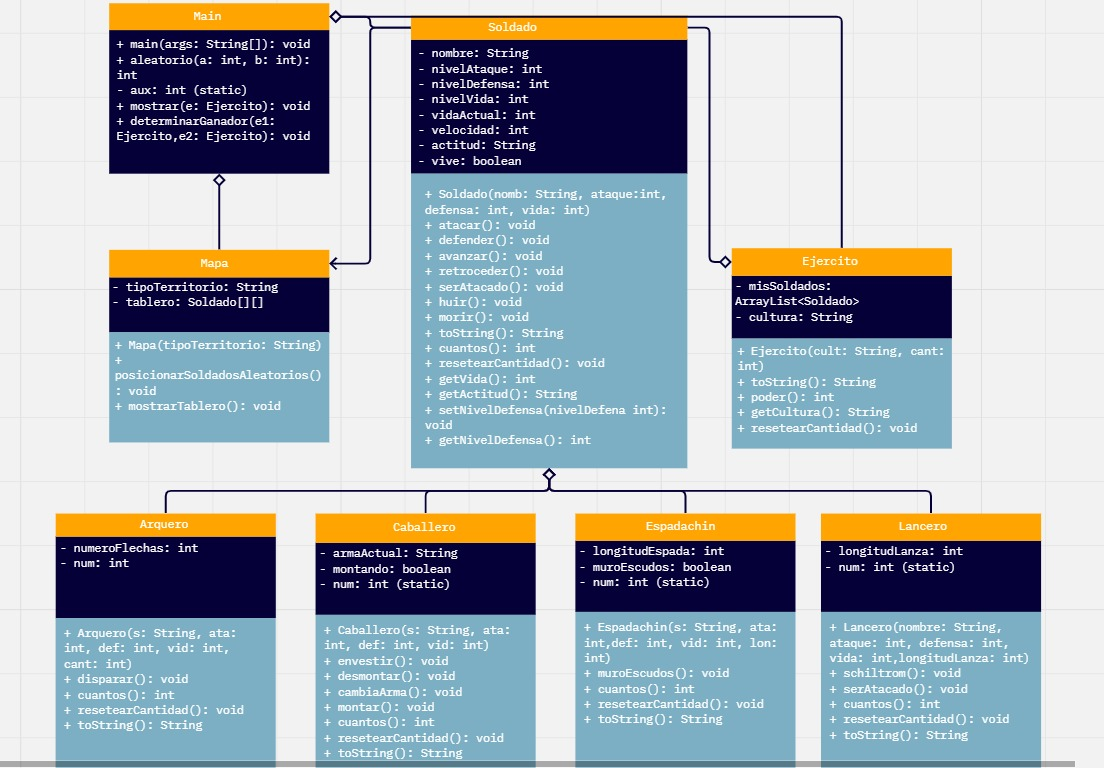
\includegraphics[height=12cm]{uml.jpeg}
        
	\end{itemize}

	\section{REFERENCIAS}
	\begin{itemize}
		\item M. Aedo, “Fundamentos de Programación 2 - Tópicos de Programación Orientada a Objetos”, Primera Edición, 2021, Editorial UNSA.
		\item \url{https://github.com/rescobedoq/programacion.git}
		\item J. Dean, "Introduction to programming with Java: A Problem Solving Approach”, Third Edition, 2021, McGraw-Hill.
        \item C. T. Wu, "An Introduction to Object-Oriented Programming with Java", Fifth Edition, 2010, McGraw-Hill.
        \item P. Deitel, "Java How to Program", Eleventh Edition, 2017, Prentice Hall.
	\end{itemize}
	
%\clearpage
%\bibliographystyle{apalike}
%\bibliographystyle{IEEEtranN}
%\bibliography{bibliography}
			
\end{document}